\documentclass[tikz,border=2pt,multi]{standalone}
\usepackage{xcolor}
\usetikzlibrary{decorations.text}

\definecolor{constraint_relaxation_color}{HTML}{cab2d6}
\definecolor{inequality_method_color}{HTML}{92b9e1}
\definecolor{mechanism_color}{HTML}{FFCCAC}
\definecolor{strategy_color}{HTML}{FFEB94}
\definecolor{subproblem_color}{HTML}{C1E1DC}
\definecolor{darkgreen}{rgb}{0, 0.5, 0}

\begin{document}
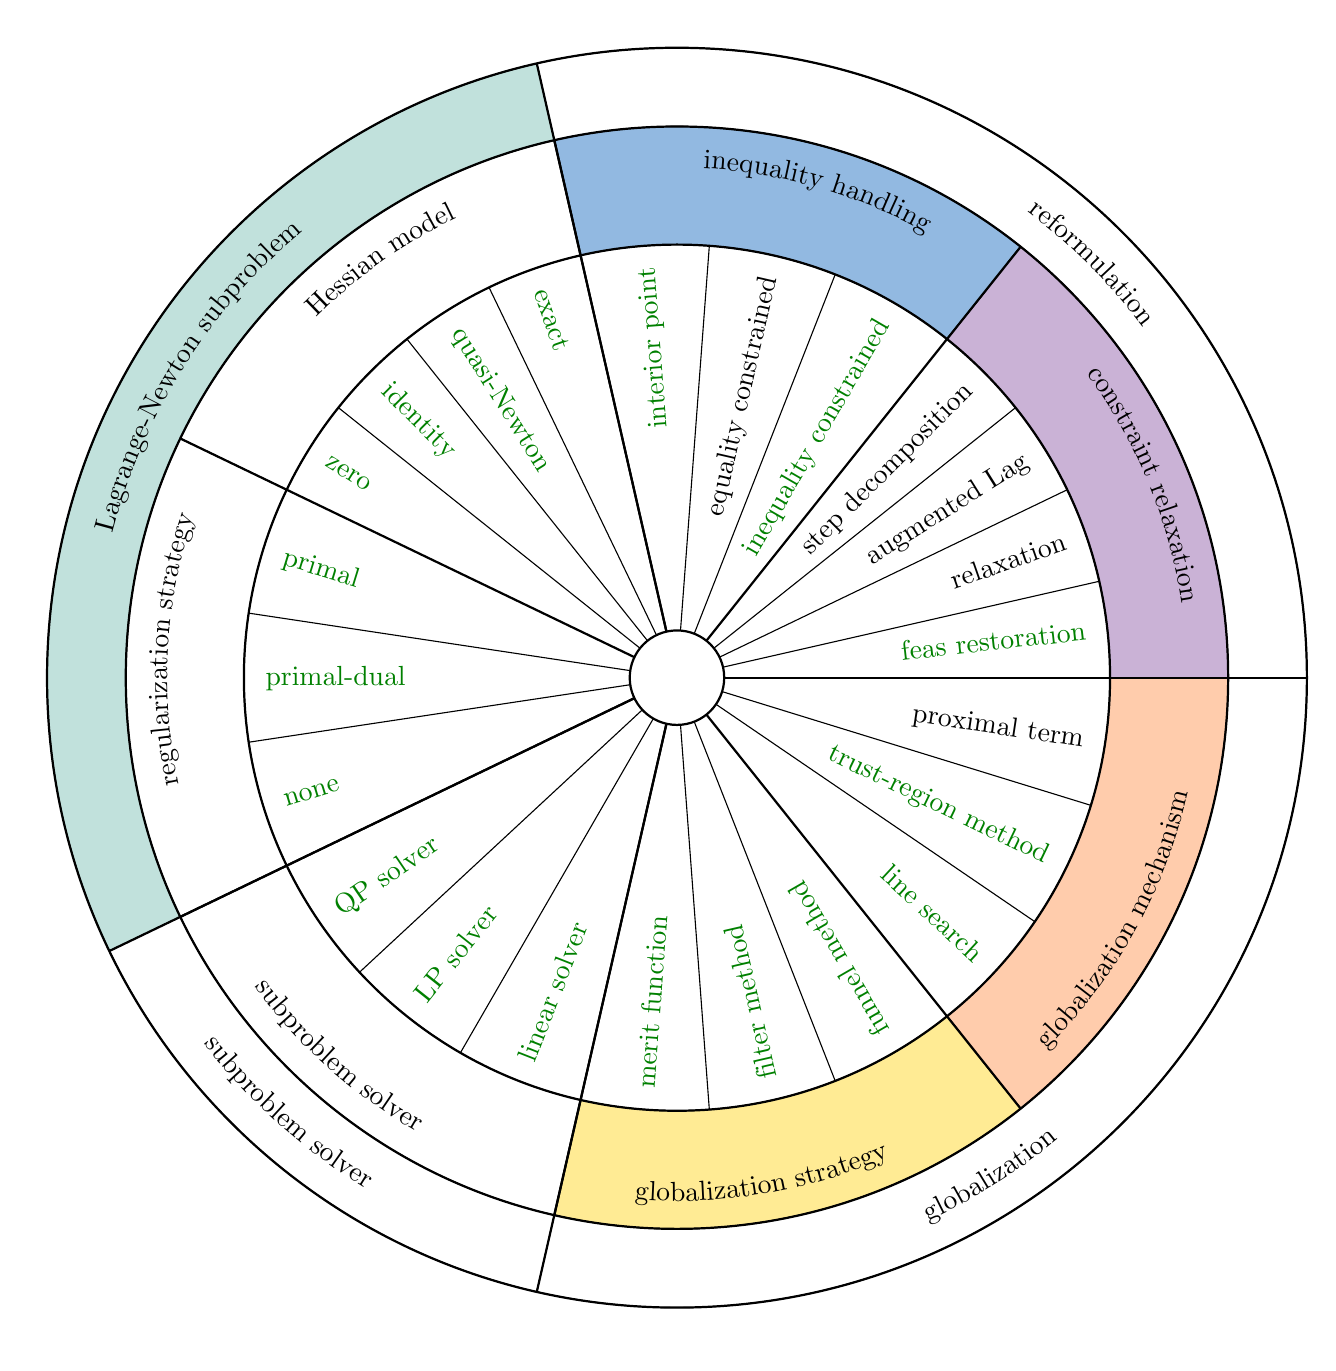
\begin{tikzpicture}
\newcommand\smallestradius{ 0.6 cm}
\newcommand\smallradius{ 5.5 cm}
\newcommand\middleradius{ 7 cm}
\newcommand\largeradius{ 8 cm}

% draw colors of layers
\filldraw[fill=white] (0: \largeradius) arc (0:102.85714285714286:\largeradius) -- (102.85714285714286: \middleradius) arc (102.85714285714286:0:\middleradius) -- cycle;
\filldraw[fill=subproblem_color] (102.85714285714286: \largeradius) arc (102.85714285714286:205.71428571428572:\largeradius) -- (205.71428571428572: \middleradius) arc (205.71428571428572:102.85714285714286:\middleradius) -- cycle;
\filldraw[fill=white] (205.71428571428572: \largeradius) arc (205.71428571428572:257.14285714285717:\largeradius) -- (257.14285714285717: \middleradius) arc (257.14285714285717:205.71428571428572:\middleradius) -- cycle;
\filldraw[fill=white] (257.14285714285717: \largeradius) arc (257.14285714285717:360.0:\largeradius) -- (360.0: \middleradius) arc (360.0:257.14285714285717:\middleradius) -- cycle;

% draw colors of ingredients
\filldraw[fill=constraint_relaxation_color] (0: \middleradius) arc (0:51.42857142857143:\middleradius) -- (51.42857142857143: \smallradius) arc (51.42857142857143:0:\smallradius) -- cycle;
\filldraw[fill=inequality_method_color] (51.42857142857143: \middleradius) arc (51.42857142857143:102.85714285714286:\middleradius) -- (102.85714285714286: \smallradius) arc (102.85714285714286:51.42857142857143:\smallradius) -- cycle;
\filldraw[fill=white] (102.85714285714286: \middleradius) arc (102.85714285714286:154.28571428571428:\middleradius) -- (154.28571428571428: \smallradius) arc (154.28571428571428:102.85714285714286:\smallradius) -- cycle;
\filldraw[fill=white] (154.28571428571428: \middleradius) arc (154.28571428571428:205.71428571428572:\middleradius) -- (205.71428571428572: \smallradius) arc (205.71428571428572:154.28571428571428:\smallradius) -- cycle;
\filldraw[fill=white] (205.71428571428572: \middleradius) arc (205.71428571428572:257.14285714285717:\middleradius) -- (257.14285714285717: \smallradius) arc (257.14285714285717:205.71428571428572:\smallradius) -- cycle;
\filldraw[fill=strategy_color] (257.14285714285717: \middleradius) arc (257.14285714285717:308.5714285714286:\middleradius) -- (308.5714285714286: \smallradius) arc (308.5714285714286:257.14285714285717:\smallradius) -- cycle;
\filldraw[fill=mechanism_color] (308.5714285714286: \middleradius) arc (308.5714285714286:360.00000000000006:\middleradius) -- (360.00000000000006: \smallradius) arc (360.00000000000006:308.5714285714286:\smallradius) -- cycle;

% draw layers
\draw [black, thick] (0:0.6) -- (0:8);
\path [decorate, decoration={text along path,, reverse path, text=reformulation, text align=center}] (0: 0.925*8) arc (0:90: 0.925*8);
\draw [black, thick] (102.85714285714286:0.6) -- (102.85714285714286:8);
\path [decorate, decoration={text along path,, reverse path, text=Lagrange-Newton subproblem, text align=center}] (102.85714285714286: 0.925*8) arc (102.85714285714286:192.85714285714286: 0.925*8);
\draw [black, thick] (205.71428571428572:0.6) -- (205.71428571428572:8);
\path [decorate, decoration={text along path, text=subproblem solver, text align=center}] (205.71428571428572: 0.95*8) arc (205.71428571428572:250.71428571428572: 0.95*8);
\draw [black, thick] (257.14285714285717:0.6) -- (257.14285714285717:8);
\path [decorate, decoration={text along path, text=globalization, text align=center}] (257.14285714285717: 0.95*8) arc (257.14285714285717:347.14285714285717: 0.95*8);

% draw ingredients
%  reformulation
\draw [black, thick] (0:0.6) -- (0:7);
\path [decorate, decoration={text along path,, reverse path, text=constraint relaxation, text align=center}] (0: 0.925*7) arc (0:{45}:0.925*7);
\draw [black, thick] (51.42857142857143:0.6) -- (51.42857142857143:7);
\path [decorate, decoration={text along path,, reverse path, text=inequality handling, text align=center}] (51.42857142857143: 0.925*7) arc (51.42857142857143:{96.42857142857143}:0.925*7);
%  Lagrange-Newton subproblem
\draw [black, thick] (102.85714285714286:0.6) -- (102.85714285714286:7);
\path [decorate, decoration={text along path,, reverse path, text=Hessian model, text align=center}] (102.85714285714286: 0.925*7) arc (102.85714285714286:{147.85714285714286}:0.925*7);
\draw [black, thick] (154.28571428571428:0.6) -- (154.28571428571428:7);
\path [decorate, decoration={text along path,, reverse path, text=regularization strategy, text align=center}] (154.28571428571428: 0.925*7) arc (154.28571428571428:{199.28571428571428}:0.925*7);
%  subproblem solver
\draw [black, thick] (205.71428571428572:0.6) -- (205.71428571428572:7);
\path [decorate, decoration={text along path, text=subproblem solver, text align=center}] (205.71428571428572: 0.95*7) arc (205.71428571428572:{250.71428571428572}:0.95*7);
%  globalization
\draw [black, thick] (257.14285714285717:0.6) -- (257.14285714285717:7);
\path [decorate, decoration={text along path, text=globalization strategy, text align=center}] (257.14285714285717: 0.95*7) arc (257.14285714285717:{302.14285714285717}:0.95*7);
\draw [black, thick] (308.5714285714286:0.6) -- (308.5714285714286:7);
\path [decorate, decoration={text along path, text=globalization mechanism, text align=center}] (308.5714285714286: 0.95*7) arc (308.5714285714286:{353.5714285714286}:0.95*7);

% draw strategy radii
%  constraint relaxation
\draw [black] (12.857142857142858:0.6) -- (12.857142857142858:5.5);
\draw [black] (25.714285714285715:0.6) -- (25.714285714285715:5.5);
\draw [black] (38.57142857142857:0.6) -- (38.57142857142857:5.5);
%  inequality handling
\draw [black] (68.57142857142857:0.6) -- (68.57142857142857:5.5);
\draw [black] (85.71428571428572:0.6) -- (85.71428571428572:5.5);
%  Hessian model
\draw [black] (115.71428571428572:0.6) -- (115.71428571428572:5.5);
\draw [black] (128.57142857142858:0.6) -- (128.57142857142858:5.5);
\draw [black] (141.42857142857144:0.6) -- (141.42857142857144:5.5);
%  regularization strategy
\draw [black] (171.42857142857142:0.6) -- (171.42857142857142:5.5);
\draw [black] (188.57142857142856:0.6) -- (188.57142857142856:5.5);
%  subproblem solver
\draw [black] (222.85714285714286:0.6) -- (222.85714285714286:5.5);
\draw [black] (240.0:0.6) -- (240.0:5.5);
%  globalization strategy
\draw [black] (274.28571428571433:0.6) -- (274.28571428571433:5.5);
\draw [black] (291.42857142857144:0.6) -- (291.42857142857144:5.5);
%  globalization mechanism
\draw [black] (325.7142857142858:0.6) -- (325.7142857142858:5.5);
\draw [black] (342.8571428571429:0.6) -- (342.8571428571429:5.5);

% draw strategies
%  constraint relaxation
\draw[white, postaction={decorate, decoration={raise=-3pt, text along path, text align=right, text={|\color{darkgreen}|feas restoration}}}] (0, 0) -- (6.428571428571429:0.95*5.5);
\draw[white, postaction={decorate, decoration={raise=-3pt, text along path, text align=right, text={relaxation}}}] (0, 0) -- (19.285714285714285:0.95*5.5);
\draw[white, postaction={decorate, decoration={raise=-3pt, text along path, text align=right, text={augmented Lag}}}] (0, 0) -- (32.142857142857146:0.95*5.5);
\draw[white, postaction={decorate, decoration={raise=-3pt, text along path, text align=right, text={step decomposition}}}] (0, 0) -- (45.0:0.95*5.5);
%  inequality handling
\draw[white, postaction={decorate, decoration={raise=-3pt, text along path, text align=right, text={|\color{darkgreen}|inequality constrained}}}] (0, 0) -- (60.0:0.95*5.5);
\draw[white, postaction={decorate, decoration={raise=-3pt, text along path, text align=right, text={equality constrained}}}] (0, 0) -- (77.14285714285714:0.95*5.5);
\draw[white, postaction={decorate, decoration={raise=-3pt, text along path, text align=right, text={|\color{darkgreen}|interior point}}}] (0, 0) -- (94.28571428571429:0.95*5.5);
%  Hessian model
\draw[white, postaction={decorate, decoration={raise=-3pt, text along path, text align=left, text={|\color{darkgreen}|exact}}}] (109.28571428571429:0.95*5.5) -- (0, 0);
\draw[white, postaction={decorate, decoration={raise=-3pt, text along path, text align=left, text={|\color{darkgreen}|quasi-Newton}}}] (122.14285714285714:0.95*5.5) -- (0, 0);
\draw[white, postaction={decorate, decoration={raise=-3pt, text along path, text align=left, text={|\color{darkgreen}|identity}}}] (135.0:0.95*5.5) -- (0, 0);
\draw[white, postaction={decorate, decoration={raise=-3pt, text along path, text align=left, text={|\color{darkgreen}|zero}}}] (147.85714285714286:0.95*5.5) -- (0, 0);
%  regularization strategy
\draw[white, postaction={decorate, decoration={raise=-3pt, text along path, text align=left, text={|\color{darkgreen}|primal}}}] (162.85714285714286:0.95*5.5) -- (0, 0);
\draw[white, postaction={decorate, decoration={raise=-3pt, text along path, text align=left, text={|\color{darkgreen}|primal-dual}}}] (180.0:0.95*5.5) -- (0, 0);
\draw[white, postaction={decorate, decoration={raise=-3pt, text along path, text align=left, text={|\color{darkgreen}|none}}}] (197.14285714285714:0.95*5.5) -- (0, 0);
%  subproblem solver
\draw[white, postaction={decorate, decoration={raise=-3pt, text along path, text align=left, text={|\color{darkgreen}|QP solver}}}] (214.2857142857143:0.95*5.5) -- (0, 0);
\draw[white, postaction={decorate, decoration={raise=-3pt, text along path, text align=left, text={|\color{darkgreen}|LP solver}}}] (231.42857142857144:0.95*5.5) -- (0, 0);
\draw[white, postaction={decorate, decoration={raise=-3pt, text along path, text align=left, text={|\color{darkgreen}|linear solver}}}] (248.57142857142858:0.95*5.5) -- (0, 0);
%  globalization strategy
\draw[white, postaction={decorate, decoration={raise=-3pt, text along path, text align=left, text={|\color{darkgreen}|merit function}}}] (265.7142857142857:0.95*5.5) -- (0, 0);
\draw[white, postaction={decorate, decoration={raise=-3pt, text along path, text align=left, text={|\color{darkgreen}|filter method}}}] (282.8571428571429:0.95*5.5) -- (0, 0);
\draw[white, postaction={decorate, decoration={raise=-3pt, text along path, text align=left, text={|\color{darkgreen}|funnel method}}}] (300.0:0.95*5.5) -- (0, 0);
%  globalization mechanism
\draw[white, postaction={decorate, decoration={raise=-3pt, text along path, text align=right, text={|\color{darkgreen}|line search}}}] (0, 0) -- (317.14285714285717:0.95*5.5);
\draw[white, postaction={decorate, decoration={raise=-3pt, text along path, text align=right, text={|\color{darkgreen}|trust-region method}}}] (0, 0) -- (334.28571428571433:0.95*5.5);
\draw[white, postaction={decorate, decoration={raise=-3pt, text along path, text align=right, text={proximal term}}}] (0, 0) -- (351.42857142857144:0.95*5.5);

% draw circles
\draw [thick] (0, 0) circle (\smallestradius);
\draw [thick] (0, 0) circle (\smallradius);
\draw [thick] (0, 0) circle (\middleradius);
\draw [thick] (0, 0) circle (\largeradius);
\end{tikzpicture}
\end{document}
